\section{Digital Design}
In this chapter the digital design will be discussed and choices will be addressed for. \\
\subsection{Finite State Machine}

The digital design was implemented with a finite state machine. The reason for this is divide the process into different states which had different functionalities. This structure would increase simplicity of the coding process. \\

The FSM has three different stages: \textbf{IDLE}, \textbf{CAPTURE} and \textbf{READOUT}. where \textbf{IDLE} is the default state for whenever no processes are running.
\begin{figure}[htp]
    \centering
    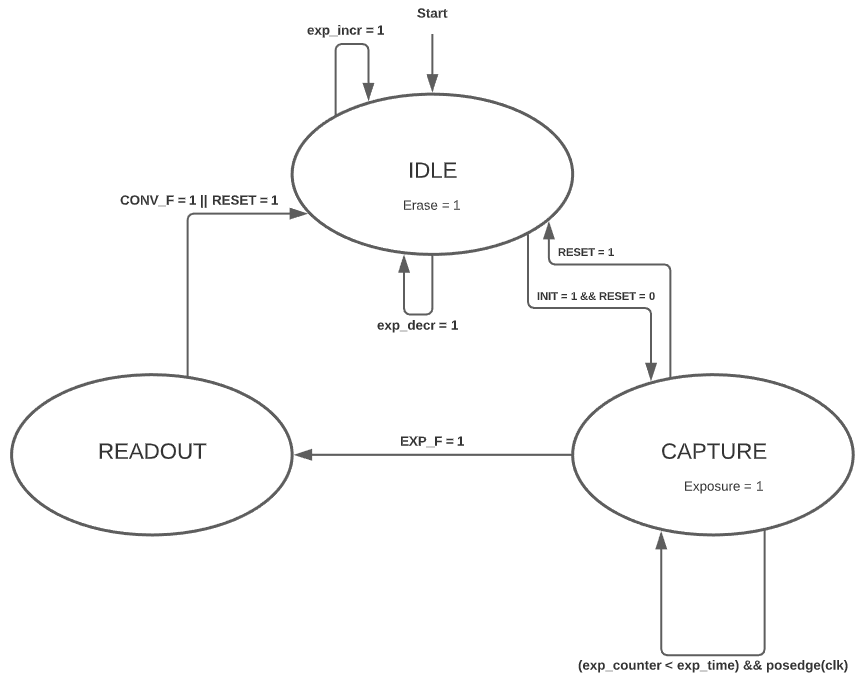
\includegraphics[scale=0.6]{Images/IC_FSM.PNG}
    \caption{FSM}
    \label{fig:FSM}
\end{figure} \\
The \textbf{READOUT} state also have some sort of FSM inside, which controls the conversation process, which is shown in figure \ref{fig:READOUT internal FSM}.
\begin{figure}[htp]
    \centering
    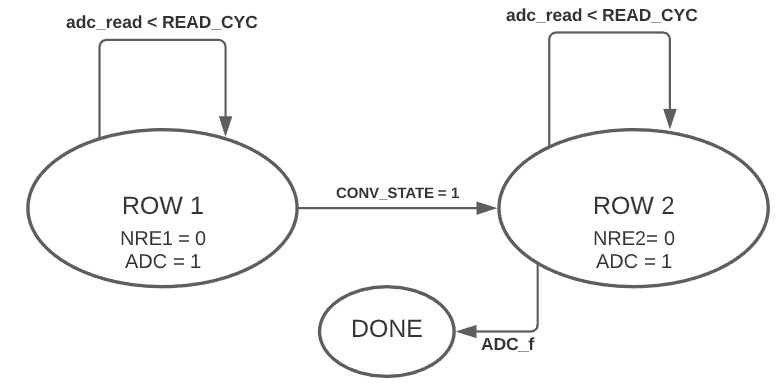
\includegraphics[scale=0.5]{Images/IC_FSM_conv.PNG}
    \caption{READOUT internal FSM}
    \label{fig:READOUT internal FSM}
\end{figure} \\
\subsection{Verilog}
The code was written in Verilog using ActiveHDL. All the Verilog code was written in the same module, because no external functions were needed. The module was first declared with the sensitivity list, and afterward the sensitivity list was defined with inputs and outputs with corresponding registers and wires. The completed program will be found in appendix \textcolor{red}{X}.





\newpage